\chapter{Introduction}
\textbf{Adarsh Pyarelal}

\section{Purpose and structure}

This document serves the purpose of declaring the following:

\begin{itemize}
    \item the capabilities we aim to demonstrate for our online agent
        components in ASIST Study 3, and how we will evaluate them.
    \item the offline analyses we plan to perform on ASIST Study 3 data
        in preparation for online deployment in Study 4.
\end{itemize}


The goal of the preregistration process as originally devised
\citep{Nosek.ea:2018} is to separate hypothesis-generating (exploratory)
research from hypothesis-testing (confirmatory) research when Null Hypothesis
Significant Testing (NHST) is used as the evaluation method. A large portion of
the activities engaged in by TA1 (Agent Architectures) performers in ASIST does
not fit neatly into the paradigm either because: (i) the `hypotheses' are about
the value of technological components (e.g., models, algorithms, and systems)
for improving the performance of artificial agents, not about theories about
the world (e.g., human behaviour) and/or (ii) the evaluation of the evidence
for or against the hypotheses is not done using NHST.

For these reasons, for each capability or analysis we declare, we also attempt
to specify what form of hypothesis is tested and what the evaluation method
will be. Our hypotheses take three forms:

\begin{enumerate}

    \item Hypotheses about \emph{technical performance} take the following form:
        Including component \emph{X} will do better for achieving \emph{Y} than
        not including \emph{X}, where \emph{X} is some technological component
        (e.g., algorithm, system component, modeling approach) and \emph{Y} is
        some specified goal such as prediction accuracy or computational
        efficiency.

    \item Hypotheses about \emph{human behavior in the context of experimental
        manipulation} take the following form: Doing \emph{X} to group A will
        predict more/less \emph{Y} compared to group B with no \emph{X}, where
        \emph{X} is an experimental manipulation applied to one group (A) but
        not to a comparison group (B) and \emph{Y} is an outcome variable
        (either latent or observed).

    \item Hypotheses about \emph{human behavior without experimental manipulation}
        take the following form: Entities (e.g., individuals, teams) with
        higher \emph{X} will do more/less \emph{Y} than entities with lower
        \emph{X}, where \emph{X} is a predictor variable (either latent or
        observed) and \emph{Y} is an outcome variable (either latent or
        observed).

\end{enumerate}

By specifying our hypotheses in one of these forms and being explicit about the
evaluation to be used for each we will achieve the central goals of
preregistration, which are avoiding post-diction and hindsight bias by not (i)
using the same data to generate and test a hypothesis, and (ii) not
``cherry-picking" results after the fact from a large set of unspecified
analyses or procedures.

Another primary motivation for this preregistration document from the
perspective of a TA1 team is to accelerate the writing of manuscripts for
publication by using the structure provided by the preregistration process to
plan ahead for publications. Each of the sections in this document is a
`component preregistation' that corresponds to a publication ‘seedling’, with
the content optimized for what we call `copy-pasteability', that is, the
ability to be copied verbatim into a manuscript for publication with minimal
changes. This is intended to reduce duplicate effort between writing up
preregistrations and publications.

Since our team is relatively large, there is little overlap in the author lists
for the individual component preregistrations. Thus, each component
preregistration has the names of the primary authors responsible for its
content section displayed under its title heading in addition to the table at
the beginning of this document. Authorship is ascribed to those who have
contributed substantially to the ideation or writing of the content.

\section{Experimental environment and task}

All the component preregistrations in this document share the same experimental
environment and task, so we describe it only once here in this section in order
to minimize redundancy.

The experimental environment is a virtual Minecraft-based testbed developed by
researchers from Aptima, Inc. and Arizona State University, who are part of the
testing and evaluation team on ASIST. 
The task is a simulated urban search and
rescue mission, in which three human participants and an AI advisor team up to
rescue victims of a building collapse. The objective of the task is to maximize
the total number of points earned by the team, where points are earned by
rescuing victims.

Each of the three human participants has a unique role
(Engineer, Medic, Transporter), and the victims can have different levels of
injury.
The task also includes perturbations in the form of threat rooms,
and unexpected rubble collapses, and mechanisms to generate interdependence
between the human teammates, thus encouraging them to communicate and
coordinate with each other.
The complete details of the experiment and task can be found in the Study 3
preregistration \cite{Huang.ea:2022}.

\section{System Overview}
\label{ch:system}

Broadly speaking, we are aiming to develop a suite of open-source technologies
for artificial social intelligence. For ASIST Study 3, we are particularly
interested in studying team coordination and communication.

For ASIST Study 3, we will deploy five containerized components. Four of them
can be classified as `analytical components' (ACs) in the parlance of the ASIST
program, and one as an `ASI', i.e. an AI agent imbued with artificial social
intelligence and designed to provide helpful interventions. In principle, the
four ACs could be bundled and deployed as part of our ASI, but we opt to keep
them separate as we expect that the resulting modularity will be beneficial for
future applications and results in additional system robustness.


\subsection{Analytical Components}

We list the analytical components we are deploying for ASIST Study 3 in
\autoref{tab:study_3_acs}. The system architecture into which they fit is shown
in \autoref{fig:nlp-architecture}.

\begin{table}
    \small
    \begin{tabularx}{5.5in}{llXl}
        \toprule
        Component           & Inputs                        & Outputs                                & Chapter\\\midrule
        ASR Agent           & Raw audio                     & Transcriptions, word-level timings     & \\
        SpeechAnalyzer      & Raw audio, transcriptions     & Sentiment and personality trait labels & \autoref{ch:sentiment_analysis}\\
        DialogAgent         & Transcriptions, chat messages & Structured events                      & \autoref{ch:rule_based_ie}\\
        DialogActClassifier & Transcriptions                & Dialog act labels                      & \autoref{ch:da_classification}\\
        \bottomrule
    \end{tabularx}
    \caption{%
        Analytical components we are deploying for ASIST Study 3, along with
        their inputs, outputs, and correspnding sections in this document that
        describe their capability in greater detail.
    }
    \label{tab:study_3_acs}
\end{table}


\begin{figure}
    \centering
    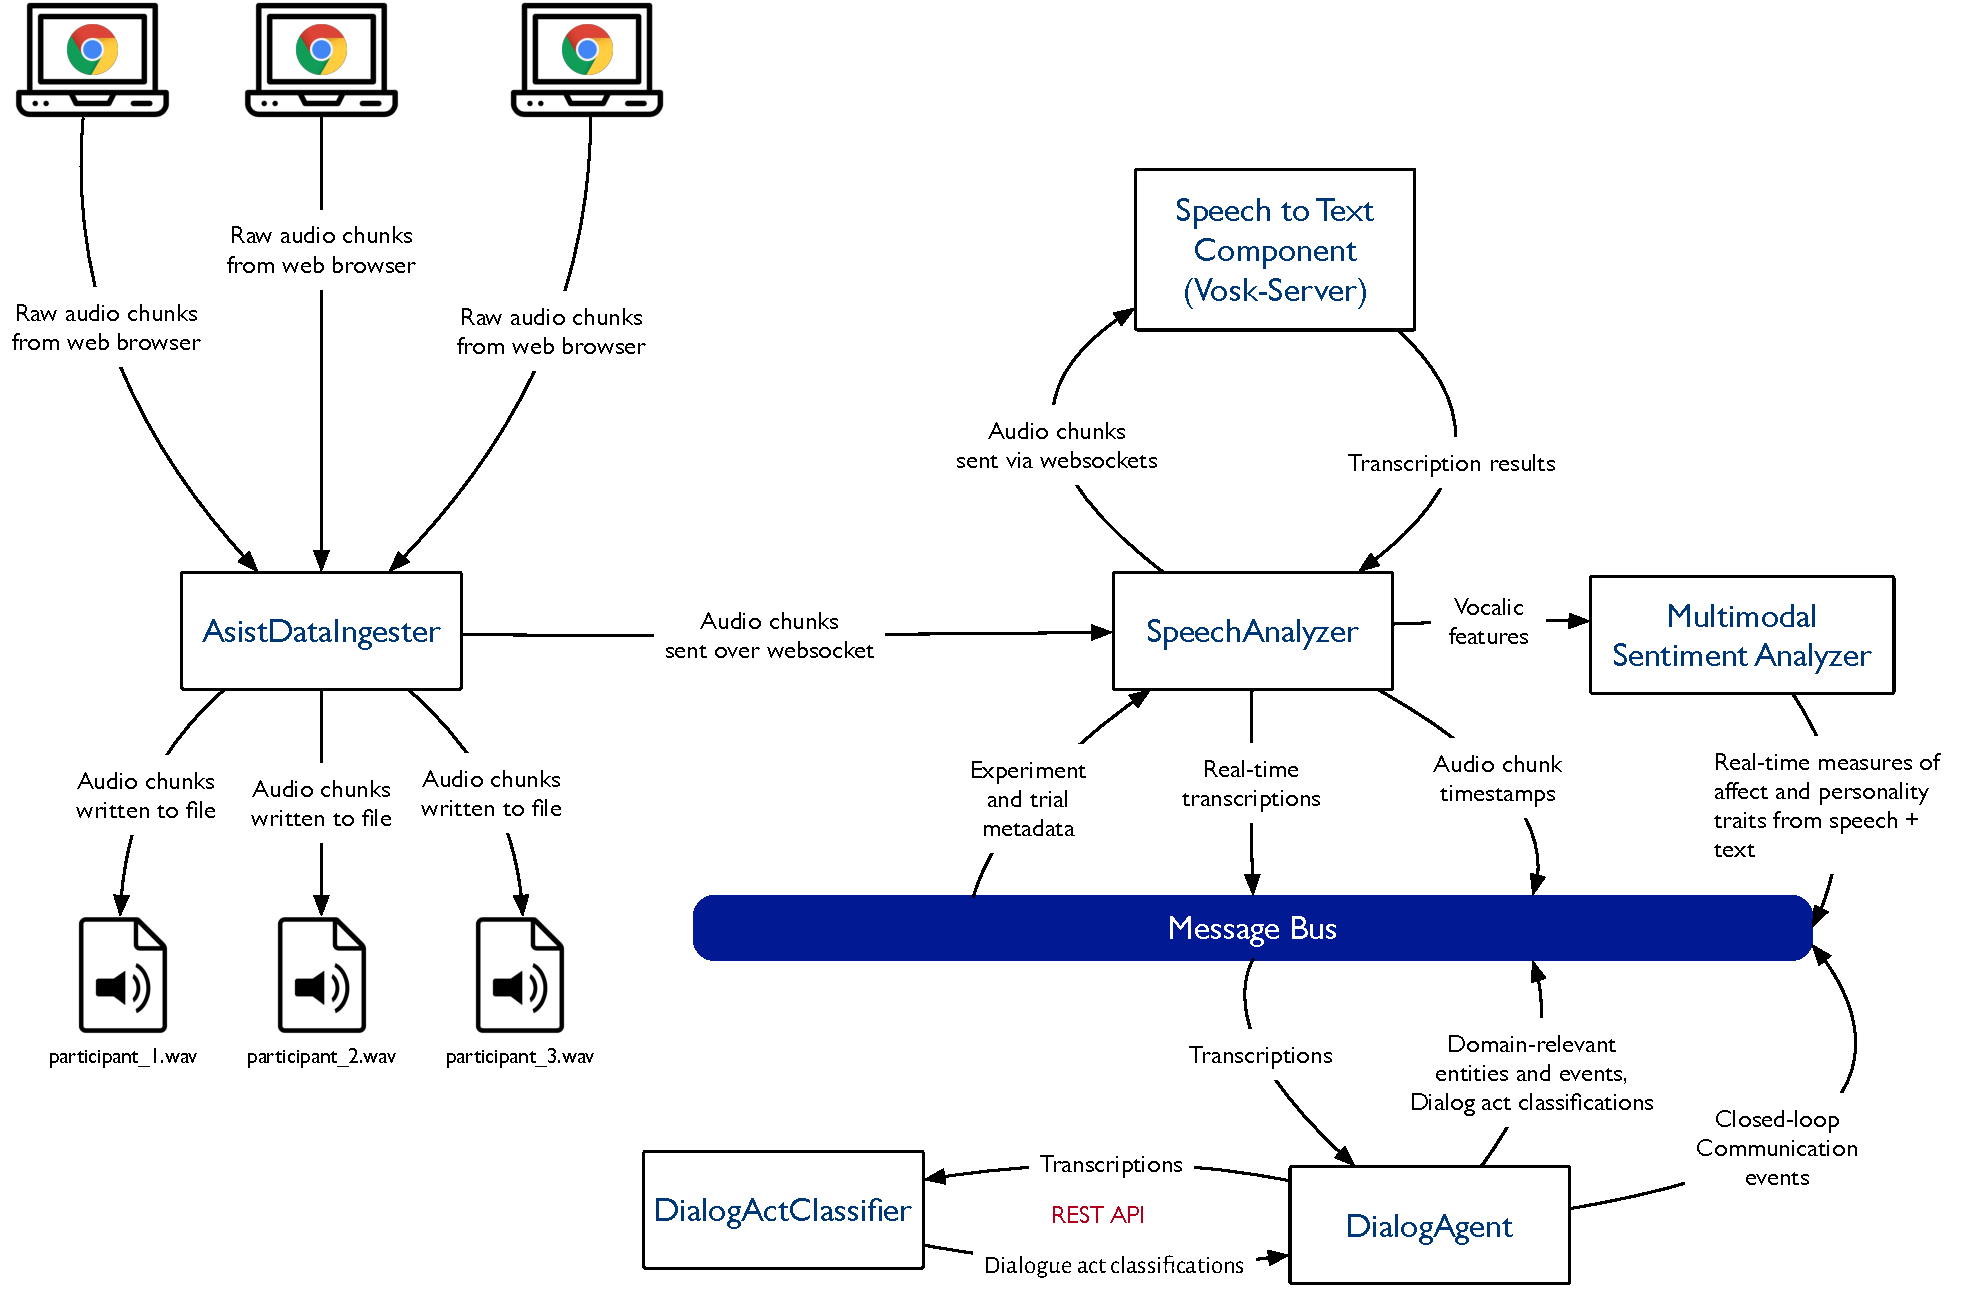
\includegraphics[width=6in]{images/nlp_architecture}
    \caption{Architecture of our multi-participant dialogue analysis system.}
    \label{fig:nlp-architecture}
\end{figure}

\subsection{Artificial Social Intelligence}

The outputs of the aforementioned analytical components are among the inputs to
our artificial social intelligence agent, ToMCAT. The core capabilities and
planned interventions of our agent are described in \autoref{ch:pgm}.

\section{Document overview}

%Give a brief summary of the preregistrations and how they contribute to the
%overall architecture.

The component preregistrations in this document span a broad spectrum of
research topics, but work together to form a cohesive suite of ASI
capabilities, with a focus on understanding and intervening on team
communication and coordination.
Each of the component preregistrations demonstrates a capability that we
believe is important for artificial social intelligence, and is currently
integrated or will be integrated in the near future into our ASI agent that
will be evaluated in ASIST study 3 or future ASIST experiments.

We begin by describing our plan for modeling team coordination and implementing
associated interventions in \autoref{ch:pgm}.  We then proceed to describe some
of the capabilities that are lower on the `software stack' that either
currently provide outputs that our AI agent or will do so in the future.

\autoref{ch:rule_based_ie} and \autoref{ch:sentiment_analysis} focus on
gleaning information from \emph{individual} natural language utterances.
\autoref{ch:rule_based_ie} discusses our rule-based system for extracting
entities and events from natural language text, and
\autoref{ch:sentiment_analysis} describes our approach to detecting sentiment
and personality traits by combining text and speech information.

In chapters \autoref{ch:da_classification} and \autoref{ch:clc}, we move beyond
analyzing utterances individually to analyzing them \emph{in context}, that is,
we consider windows containing multiple utterances to detect longer-range
phenomena. Chapter \autoref{ch:da_classification} uses context, along with
multimodal information (speech \& text) to classify dialog acts.
\autoref{ch:clc} uses explicit semantic context in utterances to automatically
detect closed-loop communication.

In \autoref{ch:entrainment}, we discuss our approach to detecting real-time
conversational alignment, or \emph{entrainment} between teammates. In
\autoref{ch:plan_recognition}, we describe our approach to multi-agent plan
recognition. \autoref{ch:question_plan} explores the connection between
question asking and inferring human plans and intentions. 

The capabilities described in \autoref{ch:clc}, \autoref{ch:entrainment},
\autoref{ch:plan_recognition}, and \autoref{ch:question_plan} will be evaluated
offline for ASIST Study 3, but we expect them to be integrated into online
components for ASIST Study 4 and future experiments.
